\documentclass[border=6pt]{standalone}\usepackage[T1]{fontenc}\usepackage{mathptmx}\usepackage{amsmath,amssymb}\usepackage{tikz}\usetikzlibrary{positioning,arrows.meta,fit,calc}\begin{document}\setlength{\columnwidth}{252pt}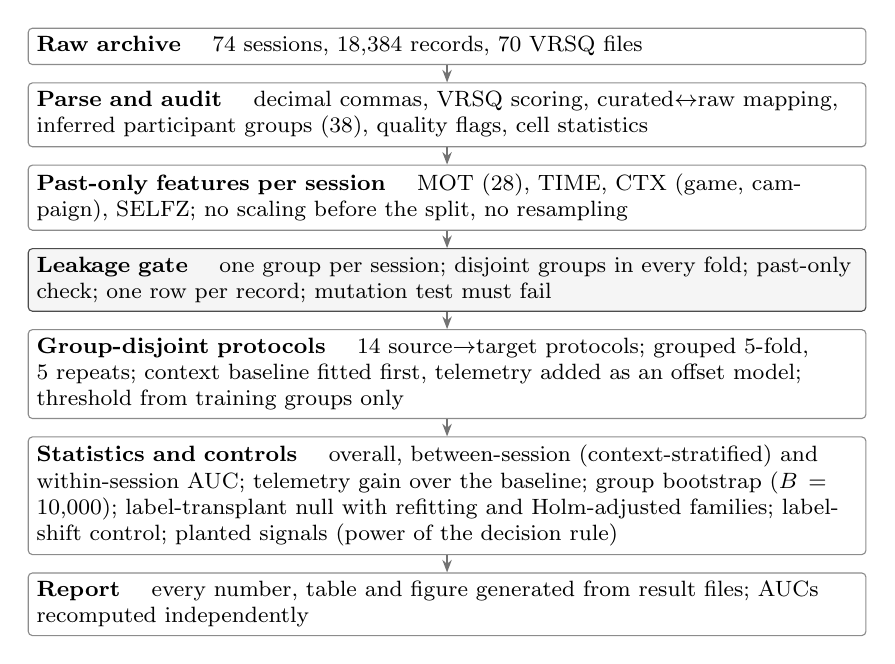
\begin{tikzpicture}[
  font=\footnotesize, node distance=2.2mm,
  box/.style={draw=black!45, rounded corners=1.5pt, align=left, inner sep=3pt, text width=0.86\columnwidth, fill=white},
  gate/.style={box, draw=black!70, fill=black!4},
  arr/.style={-{Stealth[length=1.6mm]}, draw=black!55, line width=0.5pt}]
\node[box] (raw) {\textbf{Raw archive} \quad 74 sessions, 18,384 records, 70 VRSQ files};
\node[box, below=of raw] (audit) {\textbf{Parse and audit} \quad decimal commas, VRSQ scoring, curated$\leftrightarrow$raw mapping, inferred participant groups (38), quality flags, cell statistics};
\node[box, below=of audit] (feat) {\textbf{Past-only features per session} \quad MOT (28), TIME, CTX (game, campaign), SELFZ; no scaling before the split, no resampling};
\node[gate, below=of feat] (gate) {\textbf{Leakage gate} \quad one group per session; disjoint groups in every fold; past-only check; one row per record; mutation test must fail};
\node[box, below=of gate] (eval) {\textbf{Group-disjoint protocols} \quad 14 source$\rightarrow$target protocols; grouped 5-fold, 5 repeats; context baseline fitted first, telemetry added as an offset model; threshold from training groups only};
\node[box, below=of eval] (stats) {\textbf{Statistics and controls} \quad overall, between-session (context-stratified) and within-session AUC; telemetry gain over the baseline; group bootstrap ($B=10{,}000$); label-transplant null with refitting and Holm-adjusted families; label-shift control; planted signals (power of the decision rule)};
\node[box, below=of stats] (rep) {\textbf{Report} \quad every number, table and figure generated from result files; AUCs recomputed independently};
\foreach \a/\b in {raw/audit, audit/feat, feat/gate, gate/eval, eval/stats, stats/rep} \draw[arr] (\a) -- (\b);
\end{tikzpicture}\end{document}